\section{مدیریت ریسک ها}
همیشه ریسک ها و تهدید هایی وجود داردند که بیزینس و پروژه ما را به خطر می‌اندازند. در این مرحله از مدل پیچشی سیستم توسعه، قصد داریم با ریسک های 
پروژه دست و پنجه نرم کنیم.
به این صورت که در مرحله اول انواع ریسک ها را شناسایی می‌کنیم.
در مرحله بعد آنها را بر اساس احتمال وقوع و درصد خرابی دسته بندی خواهیم کرد. در این مرحله برسی می‌کنیم که طبعات هر ریسک چه چیزی خواهد بود و چقدر نیاز است برطرف بشود.
در نهایت راهکاری پیشنهاد می‌دهیم تا به روشی خسارات ناشی از این ریسک ها را کاهش بدهیم.

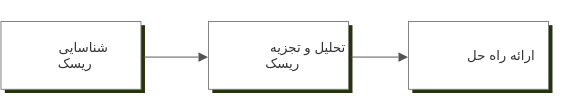
\includegraphics{assets/risk_management.png}
